% !TEX root = ../thesis.tex
\section{Doplnění řečového korpusu o specifická data - vliv nových dat na kvalitu AM}
\label{chap:realisation:corpus}

Před samotným pořízením nahrávvek promluv je nezbytné vybrat co možná nejvíce dvojic slov, které se liší významem a znělostí právě jednoho fonému. Příkladem takovýchto slov může být dvojice slov \textit{kosa} + \textit{koza} nebo \textit{přibít} + \textit{přibít}. Pro tento účel je použit algoritmus výběru slov, který je následující:

\begin{enumerate}
  \item načtení dat (slovník a hledané párové fonémy);
  \item shluknutí všech slov vedoucích ke stejné fonetické transkripci;
  \item vytvoření všech možných kombinací dvojic slovních transkripcí;
  \item nalezení dvojic transkripcí, které se liší právě ve znělosti jednoho fonému\footnote{Konkrétně algoritmus vzájemně porovná obě slova a najde rozdílné fonémy. Pokud tyto rozdíly odpovídají některé z dvojic párových fonémů, tak je dvojice přijata.};
  \item výběr dvojic slov na základě vybraných fonetických transkripcí;
\end{enumerate}

\noindent Vstupem algoritmu je \uv{slovník} obsahující slova a jejich fonetický přepis, dále pak dvojice fonémů (znělý + neznělý). Jako slovník posloužil seznam slov s fonetickými přepisy pocházející z jazykového modelu obsahující 1,2 milionu slov. Pomocí výše zmíněného algoritmu se podařilo nalézt $160$ párů slov lišících se znělostí právě jednoho fonému, celkem tedy $320$ slov. Ke každému nalezenému slovu se následně vybrala minimálně jedna věta obsahující toto slovo (ale nikoli druhé slovo z dvojice). Těchto vět je pak $418$. Příklad vybraných vět je uveden níže:

\begin{verbatim}
  Zkoušel jsem to několikrát, ale pokaždé padla kosa na kámen.
  Do basy nemusí, vlk žere, koza žije.
\end{verbatim}

Vybraná slova a věty se staly základem pro 2. etapu nahrávání. Ta se uskutečnila během dvou sezení v červenci roku 2016. Jde tedy o relativně velký časový odstup od 1. etapy. Nahrávání se zhostil stejný řečník jako v případě 1. etapy (viz část \ref{chap:construction:corpus}). Jednotlivá nahrávací sezení měla mezi sebou týdenní rozestup. Oproti 1. etapě probíhalo nahrávání v odhlučněné nahrávácí komoře a za pomocí profesionálního nahrávacího zařízení. Mikrofon byl od úst řečníka vzdálen přibližně 15 cm, protože byl použit studiový mikrofon. Ten díky své velikosti, není možné přiložit přímo na tvář jako v případě 1. etapy. K nahrávání byl použit speciální software, který kontroloval, zda každá nahrávka splňuje určité parametry. Každá akceptovaná nahrávka musí mít na svém začátku a konci minimálně $0,5\ s$ ticha a zároveň celá nahrávka nesmí být příliš tichá a zároveň přebuzená (kontrolováno pomocí energie). Pokud nahrávka nesplňuje definované parametry, je zamítnuta a řečník musí promluvu zopakovat.

V části \ref{chap:construction:corpus} je zmíněno, že je nezbytné provádět anotaci nahrávek, aby mohl být korpus kompletní. Samotná anotace je  relativně zdlouhavý proces, a proto je dobré pořídit přesné promluvy vybraných slov a vět již v průběhu nahrávání. K tomu slouží další z funkcí nahrávacího softwaru, který řečníkovi vždy ukáže text, který je potřeba vyslovit. Společně s audio záznamem je pak uložen i tento text. K dispozici je tedy nahrávka a její \uv{přepis}. Nicméně samotný řečník často může udělat chybu aniž by si toho všiml (např. záměna podobných slov apod.). Software nijak nekontroluje co je ve skutečnosti vysloveno. Z tohoto důvodu je nahrávání přítomen operátor, který poslouchá co bylo řečeno a v případě potřeby zamítné nahrávku. Řečník následně musí promluvu opakovat, dokud nahrávka neodpovídá požadovaným parametrům a zároveň je její obsah správný.

Na obr. \ref{fig:realisation:corpus:word} a \ref{fig:realisation:corpus:sentence} jsou ukázky audio záznamu slova \uv{kosa} a věty \uv{Zkoušel jsem to několikrát, ale pokaždé padla kosa na kámen.}. Pokud se nahrávky porovnají s daty získanými v 1. etapě (obr. \ref{fig:construction:el_speech}), tak hlavním rozdílem je vyšší kvalita nahrávek, zejména vyšší amplituda. Ze zobrazených spektrogramů je zřejmé, že šum je přítomen v menším množství a intenzitě než v předchozích nahrákách. Hlavní vliv na tom má nový mikrofon, který není přilepen ke tváři řečníka a nezaznamenává, tak vibrace přenášené měkkou tkání. Další rozdíl je vidět v nižších frekvencích spektrogramu, ty jsou výraznější. Přestože se jedná o stejného řečníka, tak zaznamenaná řeč nemá úplně identické parametry. Hlavním důvodem bude nepochybně změna nahrávací aparatury a procesu nahrávání. Nezanedbatelný vliv má i relativní nestálost prametrů EL řeči, zvlášť v delším časovém období. Ty jsou totiž velmi závislé na typu a pozici elektrolarynxu, ten se v době mezi nahráváními navíc změnil.

\begin{figure}[hbpt]
  \centering
  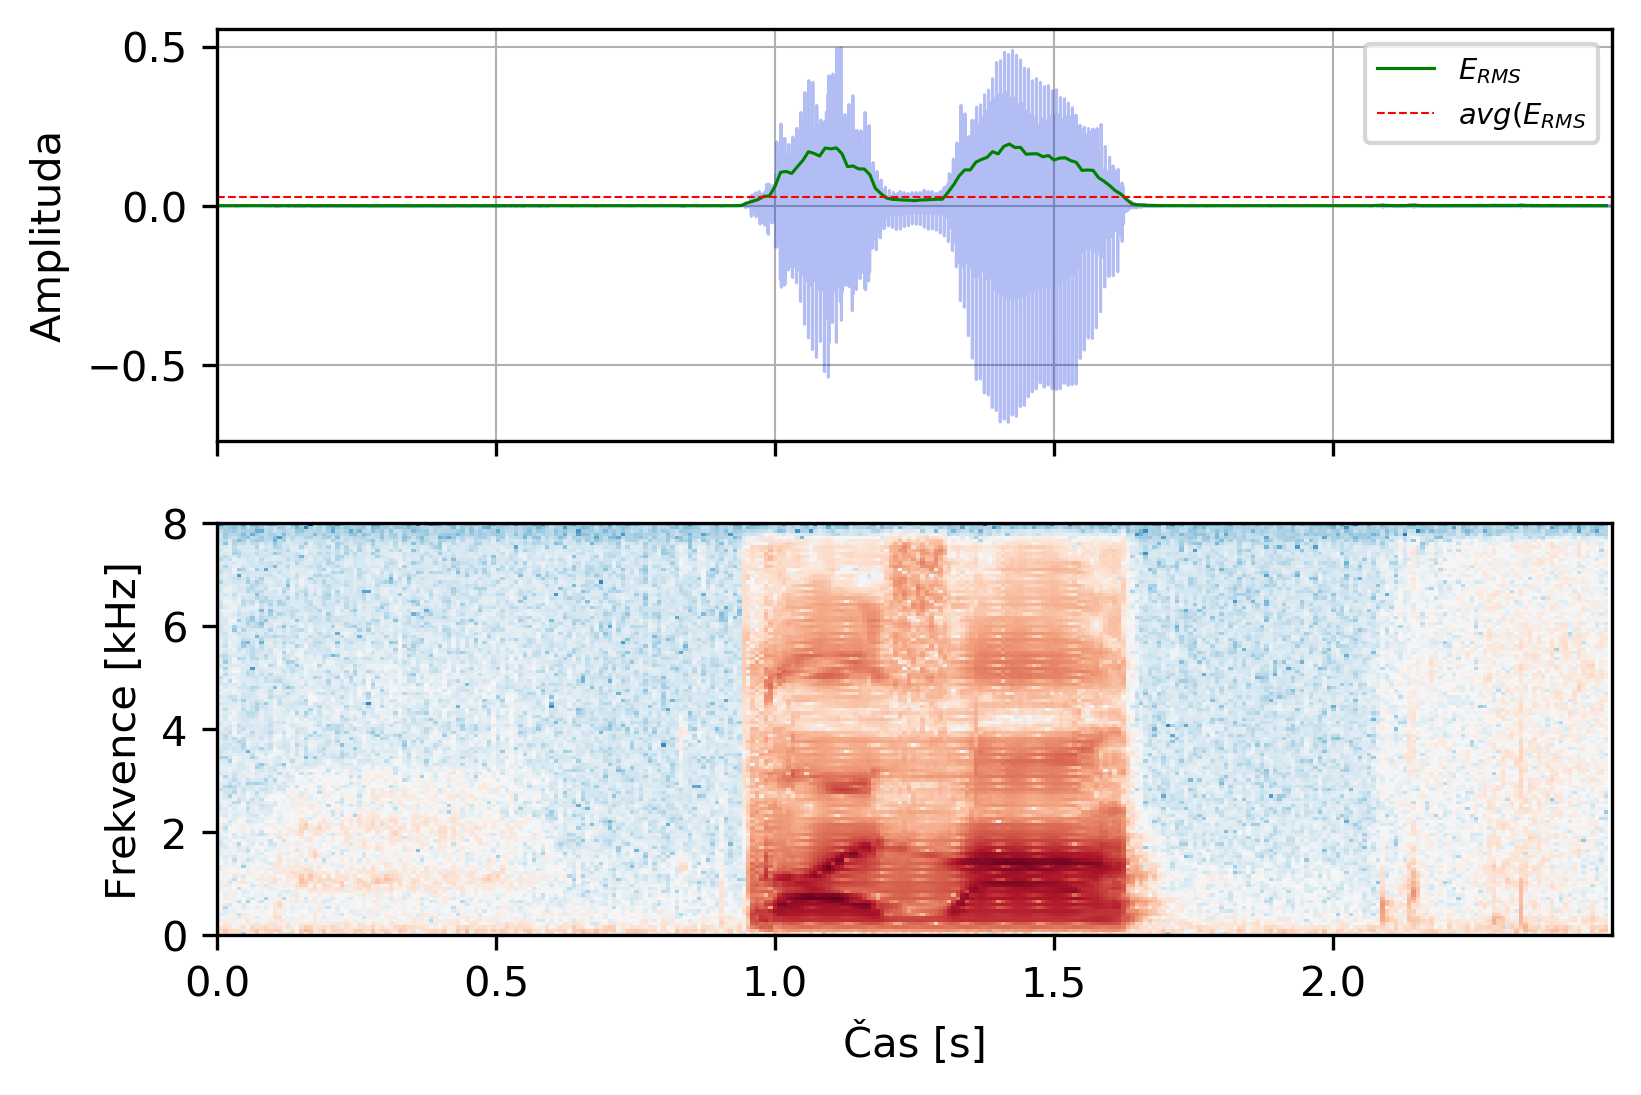
\includegraphics[width=0.9\textwidth]{./ch5-construction/img/energy_spec_word.png}
  \caption{Průběh a spektrogram slova \uv{kosa} s společně s vyznačenou energií EL promluvy.}
  \label{fig:realisation:corpus:word}
\end{figure}

\begin{figure}[hbpt]
  \centering
  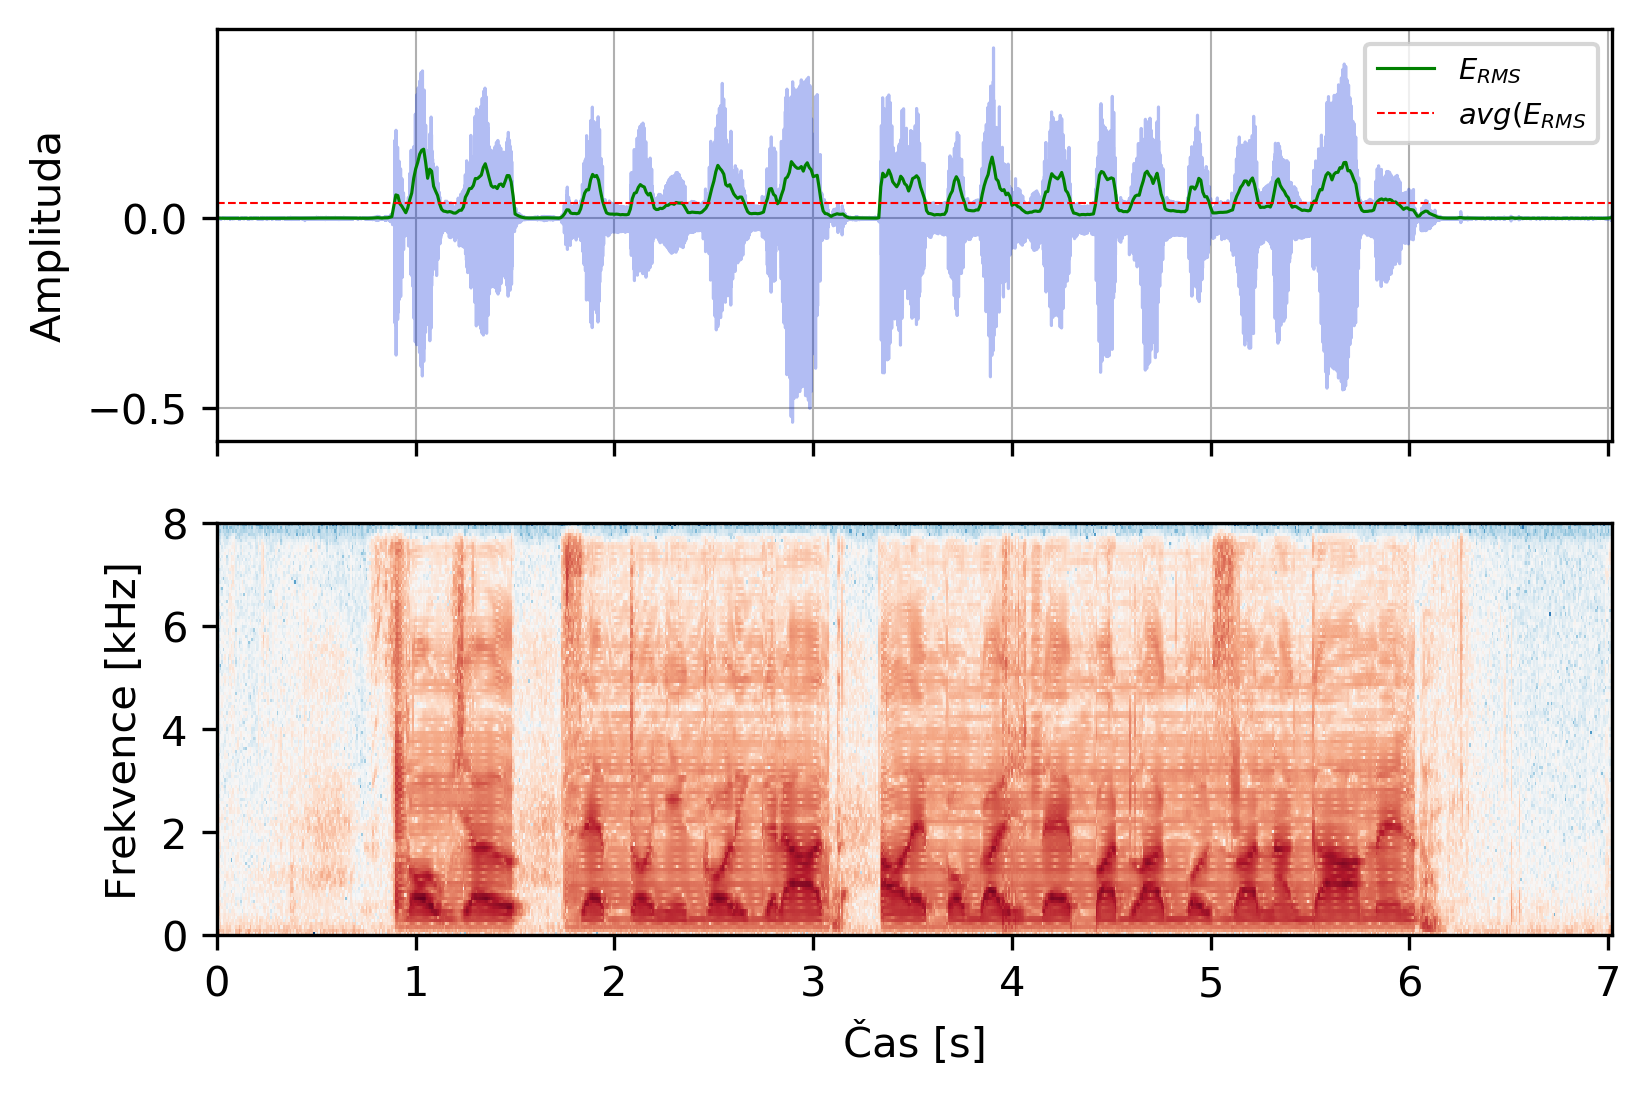
\includegraphics[width=0.9\textwidth]{./ch5-construction/img/energy_spec_sentence.png}
  \caption{Průběh a spektrogram promluvy obsahující slovo \uv{kosa} a vyznačenou energií EL promluvy.}
  \label{fig:realisation:corpus:sentence}
\end{figure}

Tab. \ref{tab:realisation:corpus:recording} přibližuje souhrnné parametry nahrávek pořízených v 2. etapě nahrávání. Celkem se podařilo získat přibližně 2 hodiny řeči (každá nahrávka obsahuje $0,5\ s$ ticha na začátku a konci). Z toho přibližně jen $10\ \%$ představují vybraná izolovaná slova. Dohromady s novými daty obsahuje korpus téměř $14$ hodin audio záznamů a k nim příslušných přepisů.

\begin{table}[htpb]
  \centering
  \def\arraystretch{1.5}
  \pgfplotstabletypeset[
    col sep=comma,
    string type,
    columns/phase/.style={column name=Nahrávání, column type={|l}},
    columns/length/.style={column name=Délka \textit{[HH:MM:SS]}, column type={|r}},
    columns/words/.style={column name=Počet slov, column type={|r}},
    columns/sentences/.style={column name=Počet vět, column type={|r}},
    columns/files/.style={column name=Počet souborů, column type={|r|}},
    every head row/.style={after row=\hline, before row=\hline},
    every last row/.style={after row=\hline},
  ]{./ch5-construction/tabs/0201-recording-stats.csv}
  \caption{Informace o korpusu nahrávek z 2. etapy nahravání.}
  \label{tab:realisation:corpus:recording}
\end{table}

\subsection{Vliv nových dat na kvalitu modelů}
\label{chap:realisation:corpus:influence}

%Mezi lety 2012 a 2016 zaznamenalo rozpoznávání řeči překotný vývoj používaných technologií. Do té doby state-of-the-art modely stavěly na kombinaci \textit{HMM} a \uv{gaussovských směsí} \textit{GMM}  U těchto modelů má každý \textit{HMM} stav svou směs, viz obr. \ref{fig:realisation:corpus:hmm:gmm}. Pravděpodobnost přechodu mezi stavy \textit{HMM} pak určují tyto směsi. Jejich parametry jsou získány na základě trénování. S příchodem open source frameworku Kaldi \cite{Kaldi2011} a rozmachem GPU výpočtů se začaly objevovat modely využívající hluboké neuronové sítě (\textit{DNN}) .

%Rozpoznávání řeči je možné si představit sequence-to-sequence modely, tedy jako převod sekvence akustických parametrů do sekvence znaků/slov. Pro tento typ úloh se a priory hodí rekurentní neuronové sítě (RNN), ale jejich slabinou je enormní výpočetní náročnost i mimo trénovací fázi a také potřeba enormního množství dat, pokud má být vytvořen end-to-end\footnote{End-to-end systémem je ve valné většině případů myšlen systém, do kterého vstupuje audio framů a  vystupuje z něj sekvence znaků. Vyvojář takového systému často nepoužívá parametrizované audio.} systém \cite{Hannun2014}. Vytvoření čistě RNN end-to-end ASR systému je tak nesmírně nákladné (data, HW, atd.). V současné době se převážně využívá kombinace \textit{HMM} modelu, který je také zástupcem rodiny sequence-to-sequence modelů, a \textit{DNN}  Hlavním rozdílem oproti těm s \textit{GMM} spočívá v tom, že pro všechny \textit{HMM} stavy se trénuje pouze jedna neuronová síť, pomocí které jsou určovány přechody mezi stavy, viz obr. \ref{fig:realisation:corpus:hmm:dnn}. Navíc tím, že tato neuronová síť určuje \uv{pouze} přechody mezi jednitlivými stavy HMM, tak může být řádově menší a jednodušší, než kdyby se jednalo o end-to-end model. Tím pádem je rychleji natrénovaná a je potřeba řádově méně dat.


% \begin{figure}[htpb]
%   \centering
%   \begin{subfigure}[b]{0.4\textwidth}
%     \includegraphics[width=\textwidth]{./ch5-construction/img/HMM-GMM.pdf}
%     \caption{HMM-GMM}
%     \label{fig:realisation:corpus:hmm:gmm}
%   \end{subfigure}
%   %
%   \begin{subfigure}[b]{0.4\textwidth}
%     \includegraphics[width=\textwidth]{./ch5-construction/img/HMM-DNN.pdf}
%     \caption{HMM-DNN}
%     \label{fig:realisation:corpus:hmm:dnn}
%   \end{subfigure}
%   \caption{Znázornění odlišného principu \textit{HMM-GMM} a \textit{HMM-DNN}.}
%   \label{fig:realisation:corpus:hmm}
% \end{figure}

% \subsubsection{Ověření přínosu nových dat}

Rozšíření korpusu umožňuje vytvoření nových modelů, které ověří konzinstenci a vliv nových dat na přesnost. Oproti baseline modelu v části \ref{chap:construction:results:baseline} jsou všechny následující modely vytvořeny ve frameworku Kaldi. Ten se po roce 2015 stal standardem pro vytváření akustických modelů, protože je velmi flexibilní a umožňuje snadné přidávání nových typů akustických modelů. \cite{Kaldi2011} Tento framework je uvolněn jako open-source.


%Oproti \ref{chap:realisation:analysis:experiment} je použit framework Kaldi, který se stal standardem pro vytváření akustikých modelů. Samotný framework se skládá z velkého množství utilit, která každá plní určitý \uv{jednoduchý} úkol v procesu vytváření a testování modelu. Kompletní proces vytváření modelu se tak sestává z postupného spouštění těchto utilit v přesně definovaném pořadí. Autoři frameworku připravili nepřeberné množství skriptů, které slouží k vytvoření různých typů modelů. Všechny modely pro EL řeč vycházejí ze skriptů pro vytvoření akustických modelů z Wall Street Journal (WSJ) korpusu. Ten je nejčastěji požíván jako jakýsi benchmark ASR systémů. Skripty jsou jen drobně upraveny, aby výsledný model pracoval s EL doménou.

Již při vytváření baseline modelu (viz část \ref{chap:construction:results:baseline}) se ukázala lepší funkce DNN modelů. Přestože vývoj výpočetních GPU postupuje závratnou rychlostí, tak natrénování HMM-DNN modelu je čásově náročnější než vytvoření HMM-GMM akustického modelu. Navíc, jak bylo popsáno v \ref{chap:asr:acoustic:DNN}, k natrénování DNN modelu je potřeba zarovnání získané pomocí HMM-GMM modelu. Proto je vhodné prvotní validaci nových dat provést na jednodušším modelu.


%Nicméně jak bylo popsáno v \ref{chap:asr:acoustic:DNN} k natrénování modelu s neuronovými sítěmi je potřeba zarovnání získané pomocí HMM-GMM modelu. Navíc natrénování HMM-DNN modelu je časově náročnější přestože vývoj výpočetních GPU postupuje závratnou rychlostí.

%Přestože \textit{DNN} nahradily \textit{GMM} v HMM, tak k jejich natrénování je nezbytné nejprve natrénovat \textit{HMM-GMM} model, který slouží k prvotnímu zarovnání (určení hranic jednotlivých fonémů v rámci audio náhrávky). To slouží jako startovní bod pro neuronovou síť. Tím, že je trénována pouze jedna síť, tak je k dispozici řádově více dat\footnote{V případě \textit{HMM-GMM} má každý stav své \textit{GMM} a tím pádem, čím více stavů, tím méně trénovacích dat pro každou směs.} k jejímu natrénování, na druhou stranu má tato síť mnohem více parametrů než všechny \textit{GMM} směsi dohromady a tak je potřeba dbát na velikost sítě. Nicméně pro standardní WSJ \textit{DNN} (6 vrstev, každá s 1024, 2048 nebo 4096 neurony) je dat dostatek.

%Přestože vývoj výpočetních GPU postupuje závratnou rychlostí, tak natrénování standardního \textit{HMM-DNN} modelu trvá o poznání déle než \textit{HMM-GMM}. Pro ověření zda je možné vytvořit model ze všech dat, která jsou k dispozici, poslouží dobře i \textit{HMM-GMM} model, který stejně slouží jako startovní bod pro \textit{HMM-DNN}, tak by se vytvářel tak jako tak. Pokud tyto modely neposkytnou \textit{DNN}  alespoň trochu \uv{dobré} počáteční podmínky, tak sofistikovanější \textit{DNN} nemusí pomoci.

Proces vytvoření akustického modelu vycházejí z předpřipravených Kaldi trénovacích skriptů pro vytvoření modelu pomocí Wall Street Journal korpusu. Tyto skripty jsou jen drobně upraveny, aby výsledný model mohl být natrénován z EL korpusu. Data jsou zparametrizována pomocí Perceptual Linear Prediction (PLP) s 12 kepstrálními, delta a delta-delta koeficienty\footnote{V rámci úpravu Kaldi skriptů se PLP parametrizace ukázala jako vhodnější pro EL řeč. Ověření proběhlo experimentálně, kdy byly vytvořeny dva identické HMM-GMM modely s 4096 stavy, ale každý byl natrénován na jinak parametrizovaných datech (MFCC a PLP). PLP model dosáhl o $1,31\ \%$ absolutně vyšší přesnost.}. Nejprve je vytvořen monofónový model, který slouží jako inciační model pro trifónové  modely, viz obr. \ref{fig:construction:results:baseline:hmm:training}.

%Tento monofónový model je speciální případ kontextově závislých modelů, bez levého a pravého (fonémového) kontextu. Následně jsou natrénovány trifónové modely. Stejně jako v experimentech provedených v části \ref{chap:realisation:analysis:experiment}, tak i zde jsou použity rozhodovací stromy, protože počet všech variant trifónů je příliš velký a dat nedostatek.

V části \ref{chap:construction:results} bylo popsáno rozdělení korpusu na trénovací a testovací sadu. Po rozšíření korpusu je rozdělení dat z 1. etapy ponecháno a nová data k jednotlivým sadám přidána. Všechny nahrané věty v 2. etapě jsou přidány do trénovací a všechna slova naopak do testovací sady. Toto rozdělení vychází z impulzu pro rozšíření korpusu o specifická slova. Ta tedy a priory mají sloužit k otestování nových podelů a tím lépe porozumnět problematice znělosti u EL řeči.

%Toto rozdělení je logické, protože důvodem rozšíření korpusu je snaha ověřit funkčnost ASR systémů na slovech, která mají rozdílný význam, ale liší se pouze znělostí jednoho fonému. Jelikož z výsledků v části \ref{chap:realisation:analysis:reduction} vyplývá, že určité spektrum trifónů je možné reprezentovat pouze pomocí znělých variant, tak při použití nahraných slov bude teoreticky možné lépe prozkoumat tuto otázku.

Jazykový model je opět fonémový zerogramový a na kompletní testovací sadě byla dosažena přesnost $ACC_{phoneme}^{GMM} = 54,96\ \%$. V případě, že testovací sada obsahovuje pouze nově nahraná slova, tak dokonce jen $ACC_{phoneme}^{GMM} = 42,97\ \%$. Což je významné zhoršení oproti výsledkům dosažených u baseline modelu v \ref{chap:construction:results:baseline} ($ACC_{phoneme}^{GMM} = 81,20\ \%$). Výpočet přesnosti je opět realizován vztahem (\ref{eq:asr:decoding:acc}).

Změna frameworku mohla zapříčinit chybu v procesu trénování. K ověření je použit křížový test, kdy pomocí stejného procesu jsou natrénovány modely z původních (1. etapa) a nových (2. etapa) dat a křížově otestovány na kompletní, původní a jen nové části testovací sady. Trénovaný akustický model má stejné parametry jako v předchozím případě. Vstupem jsou PLP data s 12 kepstrálními, delta a delta-delta koeficienty. Výsledný model může mít až 4096 stavů. Výsledky testu jsou v tab. \ref{tab:realisation:verification:cross}. Z té je jasně patrné, že trénovcací proces je \uv{správný}. Problém je tedy v datech.

%model;orig;new

\begin{table}[htpb]
  \centering
  \def\arraystretch{1.5}
  \pgfplotstabletypeset[
    col sep=semicolon,
    string type,
    columns/model/.style={column name=Model, column type={|c}},
    columns/orig/.style={column name=1. etata $[\%]$, column type={|r}},
    columns/new/.style={column name=2. etapa $[\%]$, column type={|r|}},
    every head row/.style={before row={
      \hline
      & \multicolumn{2}{c|}{Accuracy} \\
    },after row=\hline},
    every last row/.style={after row=\hline},
  ]{./ch5-construction/tabs/0202-cross_test.csv}
  \caption{Křížový test modelů natrénovaných a otestovaných na datech z 1. a 2. etapy.}
  \label{tab:realisation:verification:cross}
\end{table}

% - 20161208_param -> porovnani n vs o, vzit hodnoty z toho
% - 20170111_together -> \textit{CMN}  FULL vysledky na HMM, pak tam dat i vysledky z

\subsection{Eliminace vlivu kanálu}
\label{chap:realisation:corpus:elimination}

Z prezentovaných výsledků plyne, že nová data jsou příliš odlišná od původních a v parametrickém prostoru příliš vzdálena těm původním. Zároveň je těchto dat relativně malé množství, aby se mohly modely plně adaptovat. Na zmíněný rozdíl v datech je možné nahlížet jako na změnu kanálu, která je příčinou těchto změn. Řečník je totiž stejný. V předchozí části \ref{chap:realisation:corpus:influence} bylo zmíněno, že v rámci 2. etapy došlo ke změné nahrávací procedury a elektrolarynxu. Tím byl pozměněn kanál a logicky výsledná zaznamenaná řeč má jiné parametry než ta původní z 1. etapy. Mezi další prvky, které mohou způsobit změnu kanálu je prostředí, tedy zda je řeč produkována uvnitř nějaké místnosti, či venku, jestli je na pozadí přítomen šum atd.

K tomu, aby bylo možné použít všechna dostupná data, je tedy potřeba eliminovat vliv kanálu. K se standardně používá Cepstral Mean Normalisation \textit{CMN}. Principem této metody je odstranení vlivu kanálu na základě střední hodnoty kepstrálních koeficientů, viz dále.

Zaznamenaný signál je možné popsat jako konvoluci promluvy a vlivu kanálu, matematicky zapsáno jako

\begin{equation}
  y\left[n\right] = x\left[n\right] \circledast h\left[n\right],
  \label{eq:experiments:normalization:convolution}
\end{equation}

\noindent kde $x\left[n\right]$ představuje vstupní signál, tedy řeč, a $h\left[n\right]$ odezvu kanálu na jednotkový impulz. Zaznamenaný signál je jejich již zmíněnou lineární konvolucí. Ve frekvenční oblasti je pak rovnice (\ref{eq:experiments:normalization:convolution}) zapsaná následovně.

\begin{equation}
  Y\left[f\right] = X\left[f\right] \cdot H\left[f\right].
\end{equation}

\noindent K převodu slouží FFT. Ve frekvenční oblasti se z konvuluce stává násobení. Dalším krokem je převedení hodnot do kepstrálná oblasti. To je realizováno pomocí logaritmu spektra, stejně jako v případě MFCC parametrizace, viz \ref{chap:asr:parametrization:hearing}. V kepstrální oblasti má vzorec (\ref{eq:experiments:normalization:convolution}) následující podobu

\begin{equation}
  Y\left[q\right] = \log\left(Y\left[f\right]\right) = \log\left(X\left[f\right] \cdot H\left[f\right]\right) = X\left[q\right] + H\left[q\right],
\end{equation}

\noindent kde $q$ představuje kepstrální koeficient. V kepstrální oblasti je vliv kanálu aditivní složkou výsledného záznamu. Problémem však je, že konkrétní hodnota vlivu kanálu je neznáma. K dispozici je pouze výsledný ovlivněný signál. Předpokládejme však, že vliv kanálu je stacionární\footnote{Jedná se sice o silný, ale logický předpoklad. Pokud se vztáhne k pořízenému řečovému korpusu, tak v rámci jedné etapy nahrávání, je proces nahrávání neměnný, tzn. je použita stejná aparatura a k nahrávání dochází vždy ve stejné místnosti.}, tak poté je možné každý frame nahrávky $i$ zapsat jako

\begin{equation}
  Y_i\left[q\right] = H\left[q\right] + X_i\left[q\right],
\end{equation}

\noindent kde $Y_i\left[q\right]$ představuje $i$ frame kepstra $q$ nahrávky a $X_i\left[q\right]$ představuje $i$ frame kepstra $q$ neovlivněné řeči. Z této rovnice je pak možné vypočítat střední hodnotu

\begin{equation}
  \frac{1}{N} \sum_i Y_i\left[q\right] = H\left[q\right] + \frac{1}{N} \sum_i X_i\left[q\right].
\end{equation}

\noindent Vliv kanálu je následně možné eliminovat odečtením této střední hodnoty kepstra $q$ od aktuální hodnoty kepstra $Y_i\left[q\right]$

\begin{align}
  R_i\left[q\right] &= Y_i\left[q\right] - \dfrac{1}{N}\sum_{j} Y_j\left[q\right] \nonumber  \\
  &= H\left[q\right] + X_i\left[q\right] - \left( H\left[q\right] + \frac{1}{N} \sum_j X_j\left[q\right] \right) \nonumber  \\
  &= X_i\left[q\right] - \frac{1}{N} \sum_j X_j\left[q\right]
  \label{eq:realisation:verification:cmn}
\end{align}

\noindent S pomocí rovnice (\ref{eq:realisation:verification:cmn}) je možné odfiltrovat vliv kanálu a teoreticky tak získat nezkreslený signál. Otázkou je, přes jaký úsek počítat střední hodnotu. Je možné ji počítat přes posuvné okénko fixní délky, přes jednotlivé nahrávky, nebo dokonce přes všechny nahrávky konkrétní etapy. Pokud totiž bude uvažovaný úsek krátký, tak se může stát, že vypočtená střední hodnota nebude odpovídat skutečné střední hodnotě a tím pádem eliminace nemusí zafungovat. Vhodná délka úseku je zjištěna experimentem.

\subsubsection{Určení délky úseky pro výpočet CMN}

K určení vhodné délky úseku pro výpočet CMN je použita stejná trénovací procedura jako v předešlých experimentech s novými daty. Je tedy trénován HMM-GMM model s 4096 stavy. Vstupní data jsou parametrizována pomocí PLP. Na ně je aplikováno CMN počítáno z různé délky úseku. Celkem jsou uvažovány dva experimenty, a to

\begin{itemize}
  \item \textit{CMN} počítáno pro každou nahrávku,
  \item \textit{CMN} počítáno pro celou etapu.
\end{itemize}

V tab. \ref{tab:realisation:verification:cmn:file} jsou výsledky experimentu s \textit{CMN} počítaném přes jednotlivé nahrávky. Z dosažených výsledků je zřejmé, že je oproti výsledkům v tab. \ref{tab:realisation:verification:cross} dosaženo určitého zlepšení, zvláště pokud je model natrénován na datech z 1. etapy a otestován na datech z 2. etapy. Výsledky však nejsou zdaleka tak dobré, jako v případě trénování a testování modelu na datech ze stejné sady. Vliv tu hraje fakt, že zejména nahrávky izovlovaných slov jsou relativně krátké a vypočtené střední hodnoty, tak nabývají odličných hodnot.

\begin{table}[htpb]
  \centering
  \def\arraystretch{1.5}
  \pgfplotstabletypeset[
    col sep=semicolon,
    string type,
    columns/model/.style={column name=Model, column type={|c}},
    columns/orig/.style={column name=1. etata $[\%]$, column type={|r}},
    columns/new/.style={column name=2. etapa $[\%]$, column type={|r|}},
    every head row/.style={before row={
      \hline
      & \multicolumn{2}{c|}{Accuracy} \\
    },after row=\hline},
    every last row/.style={after row=\hline},
  ]{./ch5-construction/tabs/0203-cmn_file.csv}
  \caption{Křížový test modelů natrénovaných a otestovaných na datech z 1. a 2. etapy s \textit{CMN}  přes jednotlivé soubory.}
  \label{tab:realisation:verification:cmn:file}
\end{table}

Další experiment je s daty, kde bylo aplikováno \textit{CMN} vypočtené ze všech nahrávek konkrétní etapy. V tab. \ref{tab:realisation:verification:cmn:full} je vidět markantní zlepšení výsledků. Pokud je model natrénován na datech z 1. etapy a otestován daty z libovolné etapy, jsou dosažené výsledky velmi podobné. Nejhoršího výsledku je dosaženo, pokud je model natrénován na datech z 2. etapy a otestován na těch z 1. V tomto případě hraje velký vliv, relativně malé množství dat (pouhé 2 hodiny). Pokud je tedy \textit{CMN} počítáno přes všechny nahrávky v dané etapě, je dosaženo významného zlepšení a vliv kanálu je v podstatě eliminován. Pro doplnění je dobré zmínit, že pokud je model natrénován ze všech trénovacích dat (1. a 2. etapa) a otestován pomocí kompletní testovací sady, tak je dosažená přesnost s fonémovým zerogramovým jazykovým modelem rovna $ACC_{phoneme} = 77,69\ \%$.

%Tento výsledek je přibližující se hodnotám dosaženým v prvnotních experimentech v části \ref{chap:realisation:analysis:experiment}.

\begin{table}[htpb]
  \centering
  \def\arraystretch{1.5}
  \pgfplotstabletypeset[
    col sep=semicolon,
    string type,
    columns/model/.style={column name=Model, column type={|c}},
    columns/orig/.style={column name=1. etata $[\%]$, column type={|r}},
    columns/new/.style={column name=2. etapa $[\%]$, column type={|r|}},
    every head row/.style={before row={
      \hline
      & \multicolumn{2}{c|}{Accuracy} \\
    },after row=\hline},
    every last row/.style={after row=\hline},
  ]{./ch5-construction/tabs/0204-cmn_full.csv}
  \caption{Křížový test modelů natrénovaných a otestovaných na datech z 1. a 2. etapy s \textit{CMN}  přes všechny nahrávky v etapě.}
  \label{tab:realisation:verification:cmn:full}
\end{table}

Z výsledků v tab. \ref{tab:realisation:verification:cmn:file} je možné odvodit, že pokud by se \textit{CMN} počítalo přes posuvné okénko fixní délky, tak dosažené výsledky by nebyly zrovna dobré. Což se i experimentálně potvrdilo, když výsledná přesnost dosáhla hodnoty $ACC_{phoneme} = 56,51\ \%$ na kompletní trénovací a testovací sadě. SAmotný framework Kaldi umožňuje aplikování CMVN, což je Cepstral mean and variance normalization. Jedná se o variaci rovnice (\ref{eq:realisation:verification:cmn}), kde je kromě střední hodnoty počítána i variance. Kaldi CMVN je počítáno přes okénko fixní délky a výsledná přesnost HMM-GMM modelu s CMVN dosáhla hodnoty $ACC_{phoneme} = 76,15\ \%$ na kompletní trénovací a testovací sadě. Tento výsledek je srovnatelný s modelem využívající \textit{CMN} přes všechny nahrávky v dané etapě.

\subsubsection{Výsledky modelů po eliminaci vlivu kanálu}

Aplikací \textit{CMN} dosáhl HMM-GMM model srovnatelných výsledků jako v části \ref{chap:construction:results:baseline}. Dalším krokem je tedy natrénování HMM-DNN modelu.
%Po zjištění vhodného nastavení \textit{CMN}, je dalším krokem natrénování neuronové sítě. V předchozím textu bylo zmíněno, že neuronová síť jako počáteční podmínky používá zarovnání získané pomocí \textit{GMM}  To je získáno díky natrénovaným modelům s \textit{CMN}  přes všechny nahrávky.
Trénovaná neuronová síť FF síť má 6 vrstvev z 5 skrytých, výstupní vsrva je typu softmax s dimenzí rovnou počtu \textit{HMM} stavů. Postupně je natrénována síť s 1024, 2048 a 4096 neurony v každé vrstvě. Vstupní data jsou zparametrizována pomocí PLP s 12 kepstrálními, delta a delta-delta koeficienty a CMN počítané ze všech nahrávek dané etapy. Jazykový model je fonémový zerogramový tak, aby byl co nejvíce amplifikován vliv akustického modelu. Tab. \ref{tab:realisation:verification:dnn} zorazuje dosažené výsledky všech natrénovaných variant. Nejvyšší přesnosti dosahuje model s 4096 neurony v každé vrstvě, ale rozdíl od ostatních variant není velký. Nejlepší HMM-DNN model dosáhl $ACC_{phoneme} = 84,66\ \%$. To je zlepšení o $6,97\ \%$ absolutně oproti HMM-GMM.

\begin{table}[htpb]
  \centering
  \def\arraystretch{1.5}
  \pgfplotstabletypeset[
    col sep=semicolon,
    string type,
    columns/neurons/.style={column name=Počet neuronů, column type={|c}},
    columns/accuracy/.style={column name=Accuracy $[\%]$, column type={|r|}},
    every head row/.style={before row=\hline,after row=\hline},
    every last row/.style={after row=\hline},
  ]{./ch5-construction/tabs/0205-dnn.csv}
  \caption{Dosažená přesnost neuronové sítě s monofónovým zerogramovým jazykovám modelem.}
  \label{tab:realisation:verification:dnn}
\end{table}
